\section{Motivation}
\label{sec:motivation}
% Why is it interesting and important?
Errors in relational data are present in all fields, both in academics as well as in the industry. 

%% Industry & academics
In business, it is known throughout various studies and news articles that the cost of bad data is high. Poor data across businesses and the government cost the U.S. economy \$3.1 trillion a year in 2012 (\cite{Ilyas2015-oh}). Every company nowadays wants to be more 'data-driven', but does not foresee the challenge that arises with processing data. Also, the amount of data created and stored is growing exponentially. The total estimated amount of data stored has grown by an approximated ten-fold since 2012 and will only continue to grow according to industry experts (\autoref{fig:annual_data_size}), to an estimated 175 zettabytes\footnote{1 zettabyte = 1 billion terabytes = $10^{21}$ bytes} by 2025. This growth in data creation will lead to a growth in the amount of poor data and consequently growth in costs if not properly dealt with. 

\begin{figure}
    \centering
    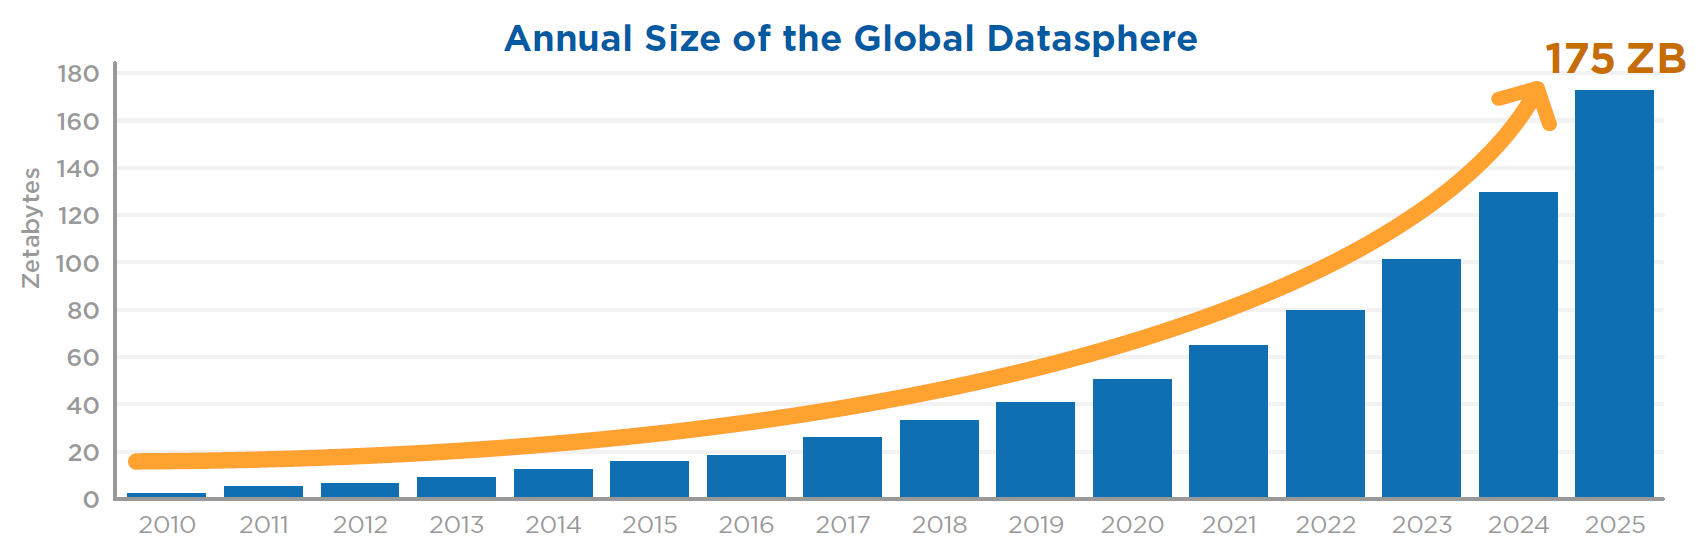
\includegraphics[width=\textwidth]{thesis/Figures/AnnualDataSize.png}
    \caption{Annual size of the global datasphere (\cite{Rydning2018-mt})}
    \label{fig:annual_data_size}
\end{figure}

% Maintain good customer relationships
% Improve organisation efficiency
% Drive useful data-driven insights
% Privacy
Companies want to use data for various reasons, such as: maintaining good customer relationships, improving organisation efficiency and drive useful data-driven insights. And at the same time following all the latest privacy regulations.  
% Pyramid of data cleaning
But, in order to pursue these aspirations and be able to extract value from data, numerous steps have to be taken beforehand. A pyramid of data science or artificial intelligence (AI) needs is shown in \autoref{fig:pyramid_data}. This shows that before any aggregating or learning from data can be done, the data needs to be explored and transformed properly. This is where error detection comes into play. If the data cleaning step with error detection as the foundation is not correctly executed, the upper levels of the data science hierarchy cannot be reached properly. Without data cleaning, valuable actions like analytics, experimentation or even artificial intelligence will not be possible.

\begin{figure}
    \centering
    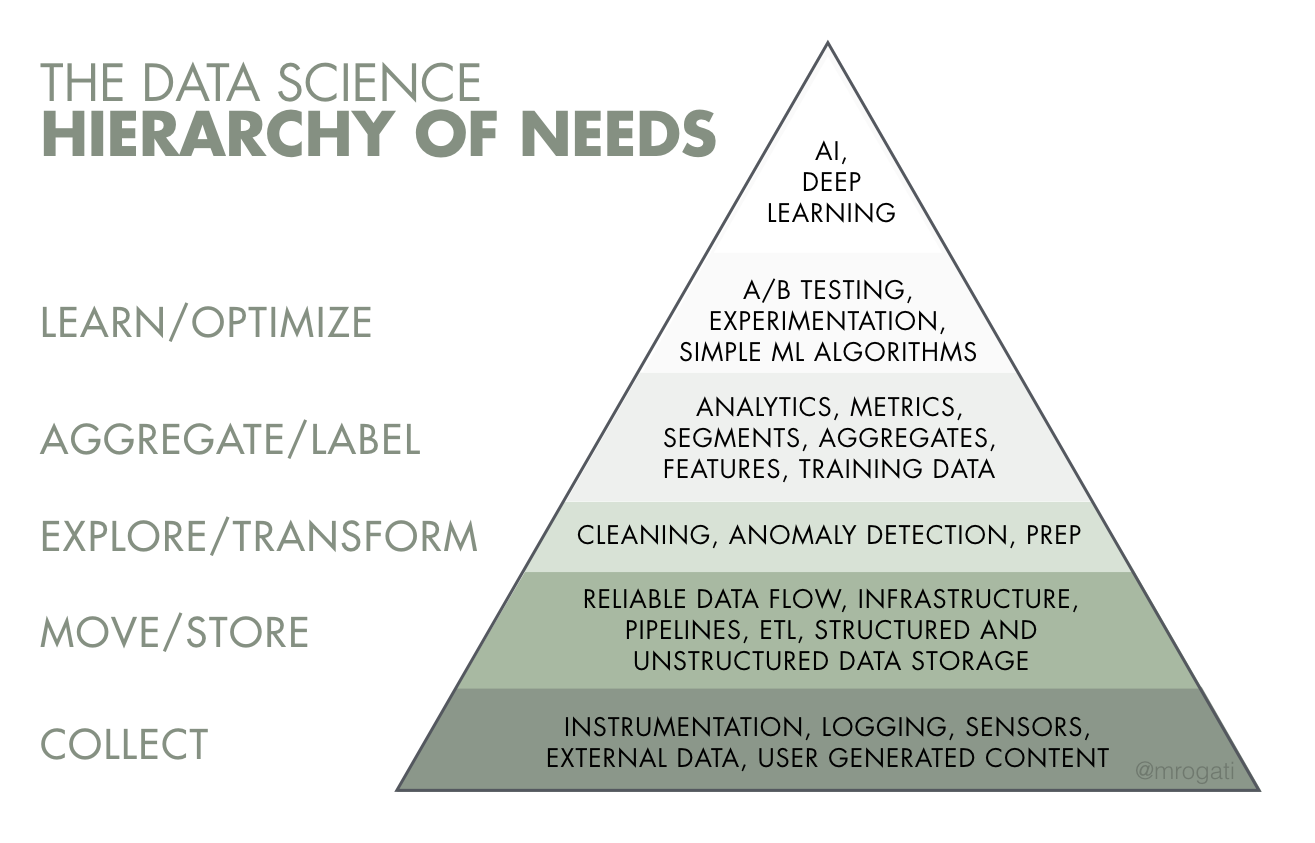
\includegraphics[width=\linewidth]{thesis/Figures/PyramidData.png}
    \caption[The data science hierarchy of needs]{The data science hierarchy of needs\footnotemark}
    \label{fig:pyramid_data}
\end{figure}
\footnotetext{Monica Rogati -  \url{https://hackernoon.com/the-ai-hierarchy-of-needs-18f111fcc007}}

% Academics focus
~\\For the past few years, governments, industry and academics have been investing both money and effort into big data and the data processing pipelines in general (\cite{Cai2015-hr}). As data quality issues in relational data sources have been a pressing problem for the industry for a longer period of time, researchers now try to take learning from experience in the field in corporate businesses (\cite{Stonebraker2018-ag}). Working with industry allows scientists to have access to more resources and real-life examples of the complications of errors in relational data, which could accelerate the solution-finding process. This is beneficial for academics, as the importance of data quality in research is also prevalent. Poor data quality might not have the monetary consequences in academics like it has in business, but bad quality in academics could lead to falsely substantiated conclusions. 

% Why is it hard? (E.g., why do naive approaches fail?)
%% Time consuming
%% Costly to run all
~\\Unfortunately, data cleaning does not have a single solution that is omnipotent and time-efficient. The complexity and heterogeneous nature of relational data make the error detection task more difficult to tackle. There is no single dominant tool for general-purpose error detection and domain-specific tools achieved better precision and recall scores than general-purpose tools (\cite{Abedjan2016-jc}). 
This leads to the difficulty of selecting the right tool for the job, with the right configuration. A user that is not familiar with the range of available options will not be able to select the best tool. Running all tools will be too time-consuming and will not have a guaranteed result. Preferably, a user wants automatic error detection, without the requirement of human expertise or any sort of configuration.

~\\If it even would be possible to provide an automatic tool, without the need of a human expert, new questions arise. 
If a machine learning (ML) model performs well, why do we not just trust the model and ignore why it made a certain decision? "The problem is that a single metric, such as classification accuracy, is an incomplete description of most real-world tasks." (\cite{Molnar2020-do}).
That is where interpretability comes into play. Not all ML systems require interpretability, but those where the problem is not studied and validated enough, or the consequences of unacceptable results are too significant need an explanation of how it works (\cite{Doshi-Velez2017-ec}). Interpret means to explain or to present in understandable terms. Because of the complexity and all different forms relational data can have, error detection in that landscape is too complex and can have too significant consequences to take its workings for granted. 

~\\Whilst there have been many solutions proposed for the task of error detection, there are still many improvements to be made. The following main problems have occurred in recent public work:

\paragraph{Usability problems:} There are many error detection tools and other data cleaning solutions that are not available to the public. Tools that are openly available have their challenges to prepare for usage in real life. Expertise is needed to configure and set up the tools. Also, the input and output formats deviate per tool. 

\paragraph{Completeness problems:} Due to the great amount of error detection tools available and the inherent costs that come with them to run, not all proposed tools in research have been tested on a broad range of datasets. Vice versa, not all types of datasets have been cleaned with the different tools available. This means that there are many unknowns when it comes to the performance of tools in all sorts of datasets or selecting the best tool for a specific dataset.

\paragraph{Interpretability problem:} All proposed tools have underlying common principles and techniques that they are designed to work with. In real-life datasets, these techniques might produce different results than expected. At the moment, no research has used interpretability methods to understand how the error detection tools work in retrospect, after evaluation. This would give better insight if and how the tools would work on unseen real-life datasets, and if there are any hidden side-effects or influences on the performance of these tools.
